\begin{table}[t]
\centering
\small
\caption{\textbf{Evaluation results for paper writing simulation.} \textit{Hard}, \textit{Medium}, and \textit{Easy} correspond to three subsets of the paper writing tasks with different difficulties, while \textit{Overall} refers to the performance across all parts. Text-embedding-large-3 is used to build embedding-based similarity metrics. Comprehensive results are available in Appendix~\S\ref{additional-exp-results}.}
\begin{tabular}{lcccc}
\toprule[1pt] 
\textbf{AGG Type} & \textbf{Easy} $\uparrow$ & \textbf{Medium} $\uparrow$ & \textbf{Hard} $\uparrow$ & \textbf{Overall} $\uparrow$ \\
\midrule
%\multicolumn{5}{c}{text-embedding-large-3 $\uparrow$} \\
%\midrule
AGG-self       & 46.42 & 45.92 & 45.90 & 46.08 \\
AGG-agent      & 56.90 & 55.55 & 53.26 & 55.24 \\
AGG-data       & \underline{74.36} & 66.42 & 56.02 & 65.30 \\
\midrule
AGG-global     & 73.79 & \underline{67.85} & \underline{60.89} & \underline{67.51} \\
%\midrule
%\multicolumn{5}{c}{voyage-3 $\uparrow$} \\
%\midrule
%AGG-self       & 52.78 & 52.60 & 53.17 & 52.85 \\
%AGG-agent      & 57.05 & 58.77 & 60.39 & 58.74 \\
%AGG-data       & 60.57 & 69.69 & \textbf{78.14} & 69.47 \\
%AGG-global     & \textbf{63.34} & \textbf{69.78} & 76.19 & \textbf{69.77} \\
\bottomrule[1pt]
\vspace{-5mm}
\end{tabular}
\label{tab:paper-writing-result}
\end{table}

\begin{table}[t]
\centering
\small
\caption{\textbf{Evaluation results for review writing simulation.} For \textit{strength} and \textit{weakness}, it shows embedding-based similarity results. We use text-embedding-large-3 as embedding models and select 5 reviewers for running \textit{AGG-agent} and \textit{AGG-global}. $\Delta\mb{S}$ refers to the average difference of review scores between real-world ones and generated ones. $\bar{\mb{S}}$ refers to the average scores of generated ones. Comprehensive results are available in Appendix~\S\ref{additional-exp-results}.}
\begin{tabular}{lccccc}
\toprule[1pt]
%\multicolumn{c}{4}{GPT-4o}
%\midrule
\textbf{AGG Type} & \textbf{Strength} $\uparrow$ & \textbf{Weakness} $\uparrow$ & $\Delta\mb{S}$ $\downarrow$ & $\bar{\mb{S}}$ \\
\midrule
%AGG-self   & 51.23/65.18          & 47.16/61.24          & 1.27 \\
%AGG-agent  & \textbf{51.66}/\textbf{66.03} & 46.75/61.29          & \textbf{1.19} \\
%AGG-data   & 51.45/65.57          & \textbf{47.62}/\textbf{61.74} & 1.26 \\
%AGG-global & 51.51/66.01          & 47.17/61.39          & 1.55 \\
AGG-self   & 51.23          & 47.16          &  1.27 & 5.33 \\
AGG-agent  & \underline{51.66} & 46.75          &  \underline{1.19} & 5.40 \\
AGG-data   & 51.45          & \underline{47.62} &  1.26 & 5.30 \\
\midrule
AGG-global & 51.51          &  47.17          &  1.55 & 5.00\\
\bottomrule[1pt]
\vspace{-8mm}
\end{tabular}
\label{tab:review-writing-result}
\end{table}


\begin{figure*}[t]
    \centering
    \begin{minipage}[t]{0.31\linewidth}
        \centering
        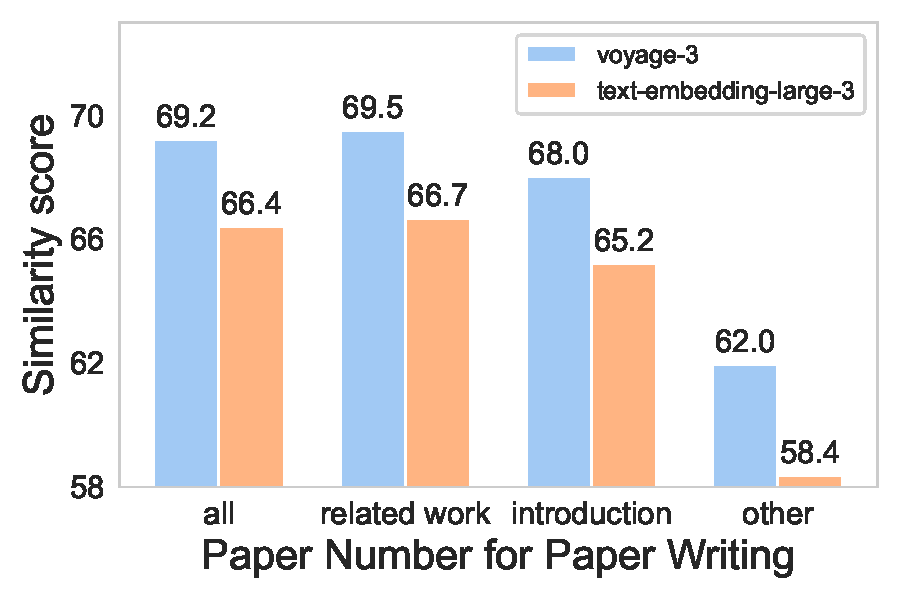
\includegraphics[width=\linewidth]{./figs/ablation_study_on_paper_number_with_seaborn.pdf}
        \par\vspace{-2.5mm}
        \caption{\textbf{Ablation study on paper number}. We select different sub-parts of cited papers in paper writing tasks.}
        \vspace{-2.5mm}
        \label{paper_writing_paper_number}
    \end{minipage}\hfill
    \begin{minipage}[t]{0.31\linewidth}
        \centering
        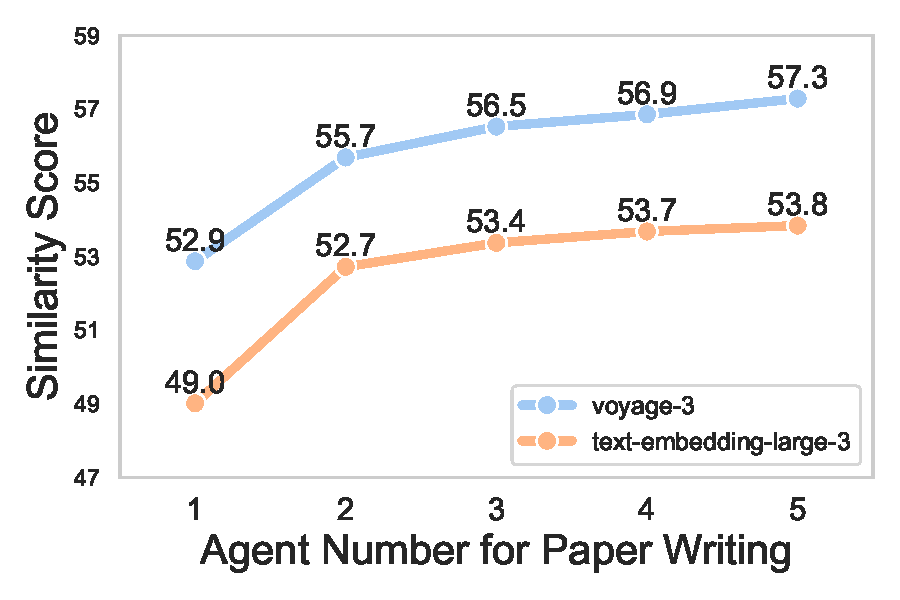
\includegraphics[width=\linewidth]{./figs/ablation_study_on_agent_number_with_seaborn_voyage.pdf}
        \par\vspace{-2.5mm}
        \caption{\textbf{Ablation study on agent number}. We select different numbers of agents for paper writing tasks.}
        \vspace{-2.5mm}
        \label{paper_writing_researcher_num}
    \end{minipage}\hfill
    \begin{minipage}[t]{0.31\linewidth}
        \centering
        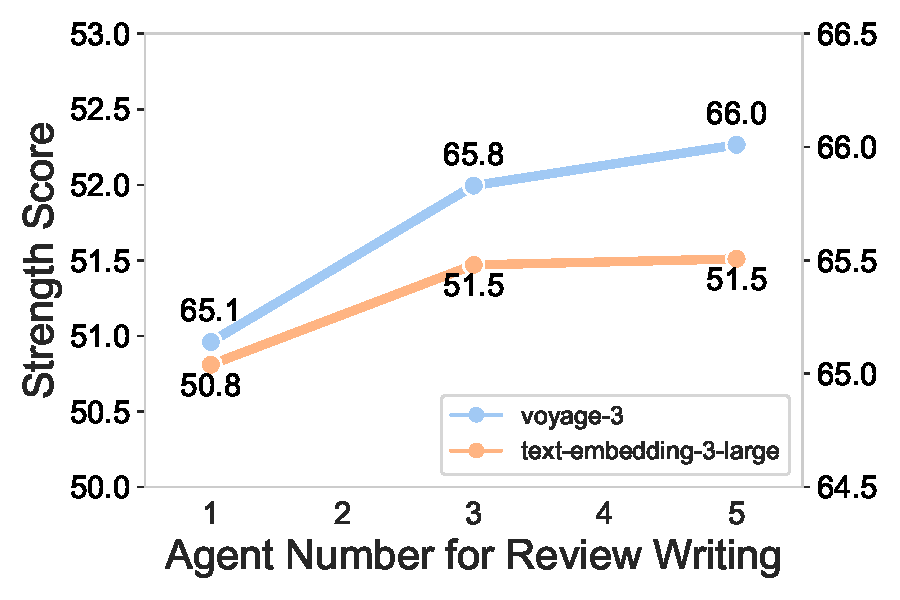
\includegraphics[width=\linewidth]{./figs/number_ablation_strength_dual_axis.pdf}
        \par\vspace{-2.5mm}
        \caption{\textbf{Ablation study on agent number}. We select different numbers of agents for review writing tasks.}
        \vspace{-2.5mm}
        \label{review_writing_researcher_num}
    \end{minipage}
\end{figure*}


\vspace{-6mm}
\section{Core Results: In-distribution Evaluation}
\label{sec:core-results}

In this section, we present the main results of our research simulation on \benchname, including 1,000 paper writing tasks and 200 review writing tasks. We evaluate existing paper nodes that have fully known their content and their neighborhoods within the community graph. We refer to these scenarios as \textit{in-distribution} cases.

\xhdr{Overall: \envname can provide a realistic simulation of research activity} To evaluate research simulation, we utilize state-of-the-art embedding models (text-embedding-3-large) to compare the semantic similarity between simulated results and real-world results. For paper writing, as shown in Table~\ref{tab:paper-writing-result}, the overall similarity score obtained using text-embedding-3-large across 1,000 papers is 67.51. Notably, the score increases to 73.79 for an easy subset of the benchmark. These results demonstrate that paper writing with \envname can produce realistic outputs compared to real-world ones. Moreover, it indicates that some ideas in top-tier conference papers are not hard to think of and can be imagined by LLMs. For review writing, as shown in Table~\ref{tab:review-writing-result}, the similarity scores are generally lower compared with paper writing, with strength-related scores averaging around 51 and weakness-related scores averaging around 47. This suggests that review writing is more challenging to generate with \envname, particularly for weakness identification. A possible explanation is that real-world review data is often noisier and more diverse, making it harder to simulate accurately.

%\xhdr{Special case: \envname can potentially come up with high-impact ideas}
%Besides the full results on \benchname, we also evaluate \envname under extreme conditions by attempting to simulate 100 of the most-cited machine learning papers from the past decade. \envname achieves low similarity scores for papers introducing groundbreaking methods, such as ``\textit{Layer Normalization}''~\citep{ba2016layer}, or novel topics, such as ``\textit{Energy and Policy Considerations for Deep Learning in NLP}''~\citep{strubell2019energy}. However, the framework performs notably better on impactful papers focused on analysis or tool development. For instance, it achieves a similarity score exceeding 0.8 for papers like ``\textit{Is BERT Really Robust? A Strong Baseline for Natural Language Attack on Text Classification and Entailment}''~\citep{jin2020bert}, which provides adversarial analysis, and ``\textit{Stanza: A Python Natural Language Processing Toolkit for Many Human Languages}''~\citep{qi2020stanza}, which offers a practical toolkit. These results suggest that high-impact research ideas may be more feasible than commonly perceived, and \envname could potentially serve as a tool to inspire future impactful research.

\xhdr{Paper writing: participation of multi-researchers improves paper quality} As shown in Table \ref{tab:paper-writing-result}, cited papers contribute more effectively than authors in the paper writing simulation, with data-aggregation achieving a score of 65.30 compared to 55.24 for agent-aggregation. The best results are obtained by combining both, surpassing data aggregation by 2.21 points. Researchers are particularly beneficial under difficult scenarios, improving the text-embedding-large-3 score from 56.02 to 60.89, likely due to the inclusion of multi-hop paper information from researchers.

\xhdr{Review writing: participation of multi-reviewers improves review quality} Unlike paper writing, review writing mainly relies on the paper that needs to be reviewed, making reviewers and cited papers less impactful, with differences limited to within 1 point. However, as shown in Table~\ref{tab:review-writing-result}, adding additional information consistently improves performance over the self-aggregation baseline. Agent aggregation performs best for writing strengths and assigning scores, while data aggregation achieves the best results for writing weaknesses. This pattern likely reflects the role of related work comparisons in highlighting weaknesses, while multiple reviewers help provide a more balanced assessment of strengths. Interestingly, global aggregation leads to larger differences in scores. We consider it an exception since GPT-4o-mini tends to apply stricter novelty judgments under global aggregation—its average assigned score drops from 5.3 to 5.0. As shown in Table~\ref{tab:model-ablation}, this effect is not observed for Qwen-2.5-7B-Instruct or Deepseek-v3, which gain better results with global aggregation.



\label{sec:underexplored-idea}
    




